%%%%%%%%%%%%%%%%%%%%%%%%%%%%%%%%%%%%%%%%%
% Short Sectioned Assignment
% LaTeX Template
% Version 1.0 (5/5/12)
%
% This template has been downloaded from:
% http://www.LaTeXTemplates.com
%
% Original author:
% Frits Wenneker (http://www.howtotex.com)
%
% License:
% CC BY-NC-SA 3.0 (http://creativecommons.org/licenses/by-nc-sa/3.0/)
%
%%%%%%%%%%%%%%%%%%%%%%%%%%%%%%%%%%%%%%%%%

%----------------------------------------------------------------------------------------
%	PACKAGES AND OTHER DOCUMENT CONFIGURATIONS
%----------------------------------------------------------------------------------------

\documentclass[paper=a4, fontsize=11pt]{scrartcl} % A4 paper and 11pt font size

\usepackage[T1]{fontenc} % Use 8-bit encoding that has 256 glyphs
%\usepackage{fourier} % Use the Adobe Utopia font for the document - comment this line to return to the LaTeX default
\usepackage[english]{babel} % English language/hyphenation
\usepackage{amsmath,amsfonts,amsthm} % Math packages

\usepackage{lipsum} % Used for inserting dummy 'Lorem ipsum' text into the template

\usepackage{sectsty} % Allows customizing section commands
\allsectionsfont{\normalfont\scshape} % Make all sections centered, the default font and small caps

\usepackage{graphicx}
\usepackage[numbered, autolinebreakds, useliterate]{mcode}

\usepackage{fancyhdr} % Custom headers and footers
\pagestyle{fancyplain} % Makes all pages in the document conform to the custom headers and footers
\fancyhead{} % No page header - if you want one, create it in the same way as the footers below
\fancyfoot[L]{} % Empty left footer
\fancyfoot[C]{} % Empty center footer
\fancyfoot[R]{\thepage} % Page numbering for right footer
\renewcommand{\headrulewidth}{0pt} % Remove header underlines
\renewcommand{\footrulewidth}{0pt} % Remove footer underlines
\setlength{\headheight}{13.6pt} % Customize the height of the header

\numberwithin{equation}{section} % Number equations within sections (i.e. 1.1, 1.2, 2.1, 2.2 instead of 1, 2, 3, 4)
\numberwithin{figure}{section} % Number figures within sections (i.e. 1.1, 1.2, 2.1, 2.2 instead of 1, 2, 3, 4)
\numberwithin{table}{section} % Number tables within sections (i.e. 1.1, 1.2, 2.1, 2.2 instead of 1, 2, 3, 4)

\setlength\parindent{0pt} % Removes all indentation from paragraphs - comment this line for an assignment with lots of text

%----------------------------------------------------------------------------------------
%	TITLE SECTION
%----------------------------------------------------------------------------------------

\newcommand{\horrule}[1]{\rule{\linewidth}{#1}} % Create horizontal rule command with 1 argument of height

\title{	
\normalfont \normalsize 
\textsc{APSC 1001, George Washington University} \\ [25pt] % Your university, school and/or department name(s)
\horrule{0.5pt} \\[0.4cm] % Thin top horizontal rule
\huge APSC 1001 Introduction to Matlab \\ % The assignment title
\horrule{2pt} \\[0.5cm] % Thick bottom horizontal rule
}

\author{\normalsize Based on "Getting Your Hands Dirty With MATLAB by Dr. Kartik Bulusu } % Your name

%\normalsize Week 1 Handout
\date{\normalsize \today } % Today's date or a custom date

\begin{document}

\maketitle % Print the title

%----------------------------------------------------------------------------------------
%	PROBLEM 1
%----------------------------------------------------------------------------------------

\section{\textbf{What is MATLAB?}}

The name MATLAB stands for MATrix LABoratory. It is a software package for numerical com-
putation and visualization with many built-in functions for technical computation, graphics and
animation. Most of these functions are state-of-the art algorithms which provide excellent tools for
linear algebra computations, data analysis, signal processing, numerical solution to ODEs etc.\\

The basic building block of MATLAB is the matrix. The fundamental data-type is the array.
Special cases of this basic data-type are vectors, scalars, real and complex matrices. In MATLAB,
you almost never have to declare the dimensions of a matrix. A novice MATLAB programmer has
to have a grasp over the basics of matrix algebra, because MATLAB quite simply and precisely
works with matrix operations.


\section{\textbf{Basics of MATLAB}}

In this section we look at the general structure of MATLAB the environment. MATLAB works through three basic windows:

\subsection{Types of Windows}

\begin{description}
\item[\textbf{Command Window:}] When you launch the MATLAB program, it pulls up this window. It is characterized by the MATLAB command prompt "\ >>\ ". All commands, including user-written pragrams, can be executed from this prompt.

\item[\textbf{Graphics Window:}] The output of all graphics commands and plotting functions are shown in the graphics window or \textit{Figure} window.

\item[\textbf{Edit Window:}] MATLAB provides a built-in editor where you can write, edit, create, and save your programs in files called \textit{"m-files"}. 
Consequently, you can use any text editor to carry out these tasks. All MATLAB programs should have a "*.m" extension. 
For example, a sample file name is "\textit{my\_program.m}".

\end{description}

There are two other important sections of the screen to be aware of:
\begin{description}
\item[\textbf{Workspace:}] The workspace is where all current variables are shown, along information about the size and type of each variable. 

\item[\textbf{Current Folder:}] Any files that you save will be located here. If you are running an .m file, it must be located in the current folder (or in the system path in MATLAB's settings).
\end{description}

\begin{figure}[h!]
\centering
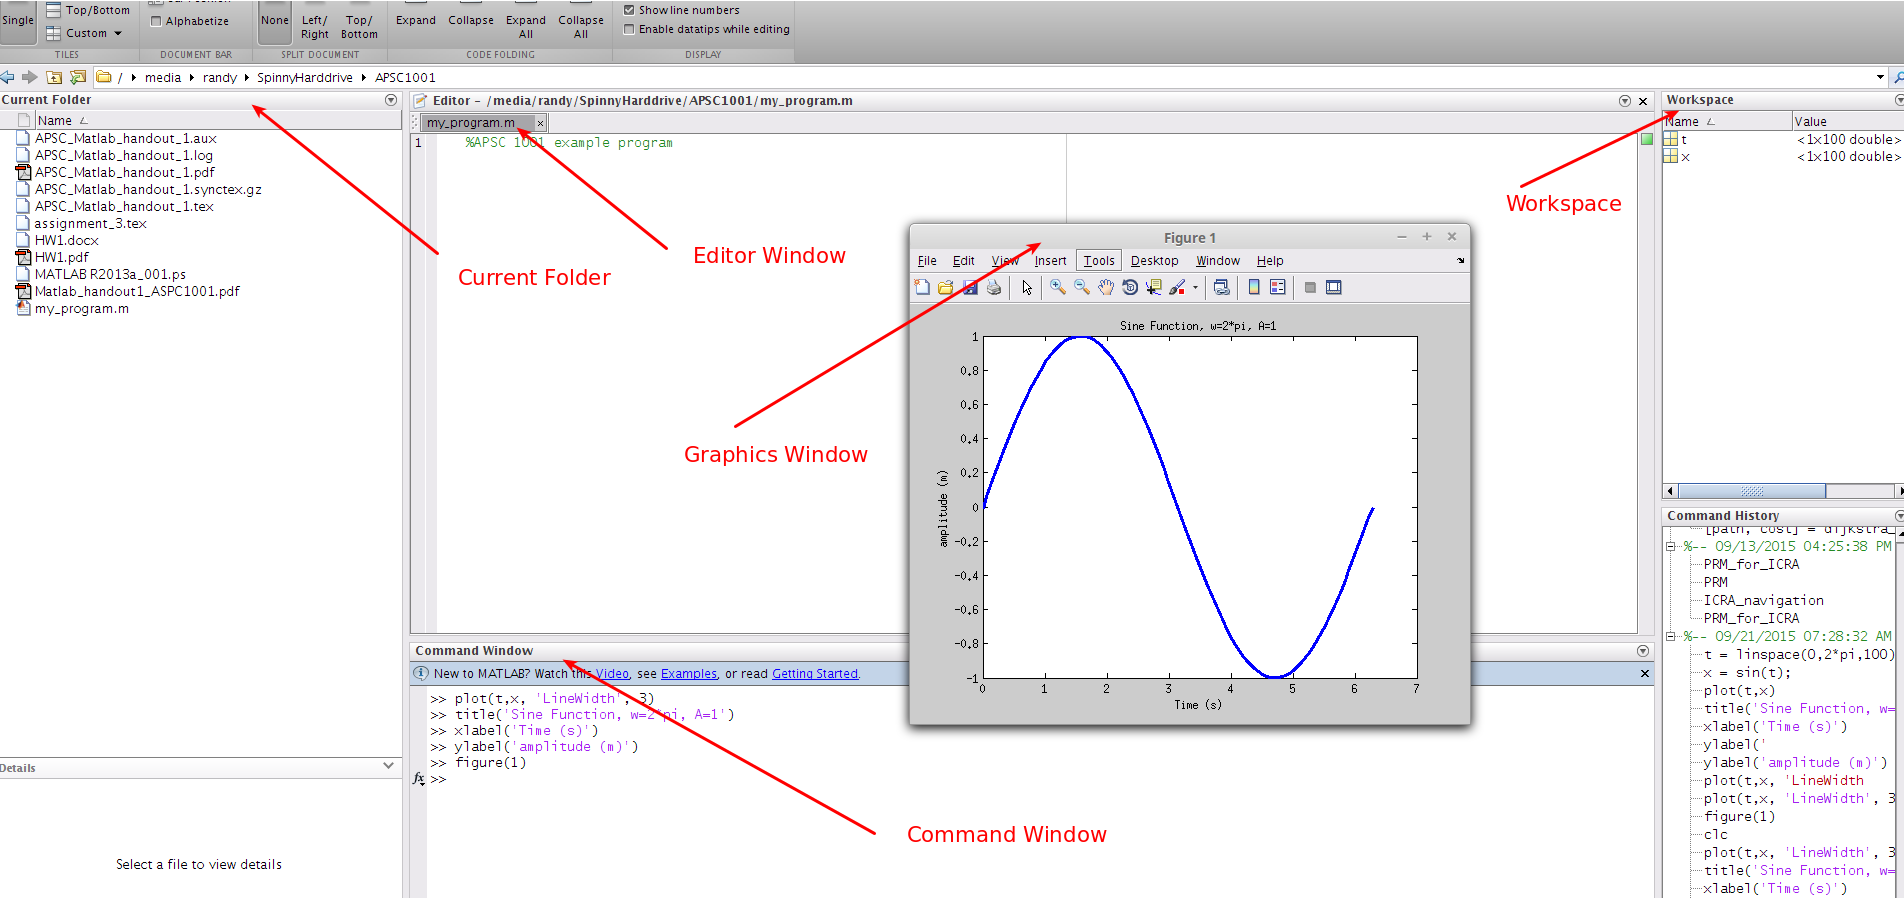
\includegraphics[scale=.25]{matlab_screenshot}
\caption{Default setup of Matlab Windows. Windows can be rearranged, minimized, or broken out if desired.}
\end{figure}

\section{Lesson 1: Creating and Working with Arrays of Numbers}

An \textit{array} is a list of numbers or expressions arranged in horizontal rows and vertical columns.
When an array has one row or column, it is called a \textit{vector.}
An array with \textit{m} rows and \textit{n} columns is called a \textit{matrix} of size $m \times n$. (Pratap, 1999) \\

There are many mathematical concepts associated with vectors and matrices that we won't cover in this course. 
Some of them you will cover in later courses, when you will appreciate that MATLAB can handle common operations such as determinant, inverse, rank, and various matrix decompositions.\\

In this lesson we deal only with one-dimensional arrays, or vectors.
In later excercises, we will introduce two-dimensional arrays, or matrices. 
Follow the instructions below and type them in the command window after you have read through the excercises.\\

Note that any text following \% symbol is a comment. 
While creating m-files or simply typing
the script on the command window any text following the \% is taken in MATLAB as comment and will not be executed in the program. 
It is a good practice to comment lines in your program so that when you revisit your code it will still make sense. 
From experience, this will save many long and painfully frustrating hours in the future.\\

\textbf{Now it's time to practice programming:}

\begin{itemize}
\item \textbf{Creating row and column vectors}
\begin{verbatim}
>>x = [2 4 5]	%x is a row vector with 3 elements
x =
 2 4 5
 
>>y = [2; 4; 5]	%y is a column vector with 3 elements
y =
 2
 4
 5 
\end{verbatim}

\item \textbf{Simple arithmetic operations on vectors}
\begin{verbatim}
>>z = [3 4 6];	 %z is a row vector with 3 elements
>>a = x + z		 %two vectors o the same size can be added or subtracted
a = 
 5 8 11
 
>>b = x + y
??? Error using ==> +
Matrix dimensions must agree.
	 %a row vector cannot be added to or subtracted from a column vector. 
\end{verbatim}

\item \textbf{Doing \textit{array} operations}
Term by term multiplication happens using the array operator, represented by a dot before the arithmetic operator (e.g. '.*').
\begin{verbatim}
	>>a = x.*z	 %multiply each term in two vectors of the same size
	%using the array operator (.*)
a = 
 6 16 30
 
	>>b = 2*a 	 %the array operator is not required to multiply by a scalar
	b=
	 12 32 60
\end{verbatim}


\item \textbf{Using trigonometric or simple math functions with array arguments}
\begin{verbatim}
>>x = [0 pi/4 pi/2];
>>y = sin(x)
y = 
 0 0.7071 1
 
>>z = sqrt(y)
z = 
 0 0.8409 1
\end{verbatim}


\end{itemize}


%----------------------------------------------------------------------------------------
\newpage
\section*{\textbf{References}}
[1] Pratap, R., \textit{Getting Started with MATLAB 5 - A Quick Introduction for Scientists and Engi-
neers}, Oxford University Press, 1999.\\

[2] Kreyszig, E., \textit{Advanced Engineering Mathematics}, 8th ed., John Wiley \& Sons, Inc., 1999.
\end{document}